\chapter{Rare Event Probabilities}\label{ch:is}
Rare events are events that occur with very low probability.
Such events can be, for example, the die-out of some population or the switching of a multimodal system across some potential barrier.
In biological applications, rare events of interest are typically related to the reachability of certain thresholds on molecule counts  or mode switching \parencite{strasser2012stability}.
By their nature, most standard methods focus on regions with high probability.
As an example consider the standard \ac{SSA}:
Trajectories are generated according to the processes density.
Therefore unlikely events are exactly as unlikely to be sampled using the direct method.
Similarly approximations such as moment approximations or mean-field analysis focus on the main probability mass.
Therefore the analysis of such events is particularly difficult.

The arguably most used method for rare event analysis is \acf{IS}.
This variance reduction method is very well-suited to the analysis of such events.
In a nutshell, this method alters the model's dynamics and keeps track of the \emph{likelihood ratio} between this altered and the original model.
This ratio provides an unbiased estimate of the event probability.
The main challenge is to find a good way to alter the model.
One popular approach is found in \acsfont{dwSSA} \parencite{kuwahara2008efficient,daigle2011automated}.
Therein each reaction rate is altered by some constant scalar factor.
These biasing values are identified by using pilot runs of the \ac{SSA} and a cross-entropy objective.
This method has been extended to be state-dependent in \citet{roh2011state}.

\section{Related Work}
\paragraph{Importance Sampling}
Most methods for the estimation of rare event probabilities  rely on  importance sampling~\parencite{kuwahara2008efficient,daigle2011automated}.

\paragraph{Importance Splitting}
Importance Splitting is an alternative Monte Carlo estimation strategy.
In this setting \emph{promising} paths are split -- initiating new simulation runs.
These runs are then reweighted according to the specific splitting algorithm.
An early proposal of the splitting technique is the \ac{RESTART} algorithm \parencite{villen1994restart}.
Further popular iterations of this idea where, for example, fixed effort and fixed success splitting \parencite{garvels1998comparison}.
For more recent developments, we refer to \parencite{budde2017better,jegourel2013importance}.
A central problem in importance splitting is determining what constitutes a \emph{promising} path.
Algorithms rely on an \emph{importance function} as an oracle.
The (approximate) backward probabilities presented here could be used as such an importance function, as well.

\paragraph{Finite state projection}
Apart from sampling-based approaches, dynamic finite-state projections have been employed by \citet{mikeev2013numerical}, but are lacking automated truncation schemes.

\section{Importance Sampling}
Importance Sampling is  a popular variance reduction technique.
\marginpar{This explanation follows \cite[Chapter~9.7]{kroese2013handbook}.}
Typically it is applied for the Monte Carlo estimation of rare event probabilities.
The main idea, is to sample from a different distribution, the \ac{IS} density, and adjust samples using the ratio between this and the original density.
Let $f$ be the original density and the goal is to estimate
\[
    \E{\theta(X)} = \int \theta(x)f(x)\,dx\,.
\]
Now let $g$ be another density, dominating $\theta f$, i.e.\ $g(x)\Rightarrow \theta(x)f(x) = 0$. Then we can re-write the above as
\[
    \expSym_f({\theta(X)}) = \int \theta(x)f(x)\,dx = \int \theta(x) \frac{f(x)}{g(x)} g(x) dx = \expSym_g \theta(X) \frac{f(X)}{g(X)}\,.
\]
Therefore, we can replace the estimate using sampling from $f$ by an estimate using the density $g$ instead.
According to the right-hand side of this equation, the estimate using i.i.d.\ samples $X_i$, $1\leq i \leq N$
\begin{equation}\label{eq:imp_sampl}
    \hat{\expSym}(\theta(X)) = N^{-1} \sum_{k=1}^N \theta(X_k) \frac{f(X_k)}{g(X_k)}\,.
\end{equation}
The term factor
\[
    W(x) = \frac{f(x)}{g(x)}
\]
is called the \emph{likelihood ratio}.

Thus, the method hinges on finding a density $g^{*}$, that has a computable likelihood ratio and  minimizes the variance of the estimator \eqref{eq:imp_sampl}.
If $\theta(x)$ is an event, the perfect \ac{IS} \parencite[Chapter~9.7.1]{kroese2013handbook}
\[
    g^*(x) = \frac{\theta(x) f(x)}{\E{\theta(x)}}\,.
\]
Therefore the ideal \ac{IS} distribution is the conditional density
\[
    g^*(x) = f(x \mid \theta(X) = 1)\,.
\]

\section{Near-Optimal Biasing}
An \ac{MPM} can be modified to fullfill terminal constraints.
Previously, in \autoref{sec:bridge_dist}, we have seen how the endpoint constrained process can be described using the backward probabilities $\beta$.
The bridging distribution can be either computed using both backward and forward probabilities, but for us it is more instructive to consider, the bridging \ac{CME}.
This is the endpoint constrainted version of the \ac{CME}.
It depends on ratios of the backwards probabilities which act as factors to the propensity values.
Taking the derivative of $\gamma(x,t)=\pi(x,t)\beta(x,t)$, yields the bridging \ac{CME} (see also \citet{huang2016reconstructing})
\begin{equation}\label{eq:bridge_cme}
    \frac{d\gamma}{d t} ( x,t) =
    \sum_{j=1}^{n_R}\left(
        \tilde{\alpha}_j( x- v_j)\gamma( x- v_j,t) - \tilde{\alpha}_j( x)\gamma( x,t)
    \right)\,,
\end{equation}
where the propensities
\begin{equation}
    \tilde{\alpha}_j(x, t) = \alpha_j(x)\phi_j(x, t)\,.
\end{equation}
The time-dependent predilection factor
\begin{equation}\label{eq:dyn_predilection}
    \phi_j(x, t) = {\beta(x + v_j, t)}/{\beta(x, t)}\,.
\end{equation}
Equation~\eqref{eq:bridge_cme} reveals the optimal biasing scheme for \ac{IS}.
Since, we know that the ideal \ac{IS} distribution is the conditional distribution $\gamma$, the ratios
give a perfect biasing.
We use approximations of these ratios as a time and state dependent predilection functions $\phi_j$ during the stochastic simulation.

Naturally, computing \eqref{eq:bridge_cme} requires full knowledge of all backward probabilities $\beta(x, t)$ for all states $x$ and times $t$.
A full backward solution contains more information than the event probability, we are interested in.
In particular, the event probability is precisely $\beta(x_0, 0)$.
To make this approach feasible, we will use the aggregation-based approximation $\hat{\beta}$ of the backward probabilities $\beta$.
Thus, we will compute and store backward probabilities for the aggregated system for discrete time points up to $T$.
\[
    \bar{\phi}(i, j; t) = \hat{\beta}\left(\bar{x}_j, \Delta\floor*{\frac{t}{\Delta}}\right) / \hat{\beta}\left(\bar{x}_i, \Delta\floor*{\frac{t}{\Delta}}\right)
\]
Using these approximate backwards probabilities we can compute approximate predilections for the aggregated system.

In \autoref{fig:biases} we illustrate this scheme for a birth-death process (\autoref{model:bd}) with goal macro-state $[40,47]$ at $T=10$
and $X_0=0$.
\begin{figure}
    \centering
    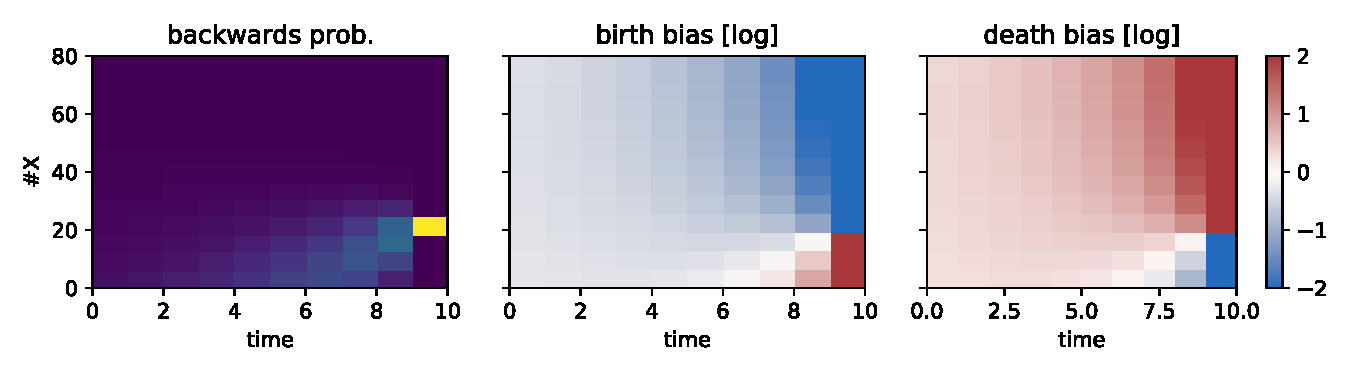
\includegraphics[width=\textwidth]{gfx/biases.pdf}
    \caption[Approximate biasing]{\label{fig:biases}The approximate dynamic biasing (cut to $[e^{-2}, e^{2}]$) illustrated for a birth death process with macro-state size $8$ and target state $[40, 47]$ at $T=10$ for $10$ time points.}
\end{figure}
\autoref{fig:biases} clearly illustrates how the biases increase towards the end increasing the push towards the goal state the farther time progresses.
Since by the approximation assumption, all constituent states of a macro-state are treated as equivalent, the macro-state biases are transferred to the micro-states.
Depending on the scenario, this interpolation could be replaced by other schemes, such as nearest neighbor interpolations.
In fact, such an approach might be better suited in the example above, where we aim to push the process to a specific micro-state.

The discrete steps in the time domain are kept.
This enables the application of an adjusted \ac{SSA} that can deal with piecewise constant rate functions in the waiting time distributions.
This algorithm is discussed in the following section.

\section{Non-homogeneous Stochastic Simulation}
We are changing the rate bias dynamically over fixed intervals of the time-domain.
Therefore we cannot use the default \ac{SSA}.
With \autoref{alg:ssa_dyn} we present a version of the \acl{SSA} that simulates trajectories of a system with such dynamically changing biases.
The main change is the handling of the time-discrete changes in the loop in \autoref{line:tloop}.
Here it is tested, in which time interval the sampled jump will take place.
Therefore rates are recomputed each time the algorithm jumps forward one time-interval.

Let us first consider how exactly the jump time distribution changes.
A time-inhomogeneous exponential has the cdf
\[
    F(t) = 1 - \exp\left(-\int_0^t \lambda(s)\,ds\right)\,.
\]
Accordingly, the pdf
\[
    f(t) = \lambda(t)\exp\left(-\int_0^t \lambda(s)\,ds\right)\,.
\]
Since we compute the biases for fixed intervals, we have an exponential model with a piecewise constant rate function.
In \autoref{fig:bias_ssa:pce}, we give an example of such a distribution.
Assume, we have an increasing sequence of time points $\tau_0=0, \tau_1, \tau_2, \tau_3, \dots$ with corresponding rates $\lambda_i >0$.
The piecewise constant hazard function
\[
    \lambda(t) = \begin{cases}
        \lambda_1, & \text{if } \tau_0 \leq t \leq \tau_1\\
        \lambda_2, & \text{if } \tau_1 < t \leq \tau_2\\
        \lambda_3, & \text{if } \tau_2 < t \leq \tau_3\\
        \quad\vdots
    \end{cases}\,.
\]
We can give the pdf using a case distinction as
\begin{equation}
    f(t) = \begin{cases}
        f_1(t), & \text{if }\tau_0 \leq t \leq \tau_1\\
        f_2(t), & \text{if }\tau_1 < t \leq \tau_2\\
        f_3(t), & \text{if }\tau_2 < t \leq \tau_3\\
        \quad\vdots
    \end{cases}\,,
\end{equation}
where, letting $\Delta_k = \tau_k - \tau_{k-1}$, the piecewise densities
\[
    f_k(t) = \lambda_k \exp \left( -\sum_{i=1}^{k-1}\Delta_i\lambda_i - \lambda_k\left(t - \tau_{k-1}\right)\right)\,.
\]
Similarly, the cdf
\begin{equation}
    F(t) = 1 - \begin{cases}
        S_1(t), & \text{if }\tau_0 \leq t \leq \tau_1\\
        S_2(t), & \text{if }\tau_1 < t \leq \tau_2\\
        S_3(t), & \text{if }\tau_2 < t \leq \tau_3\\
        \quad\vdots
    \end{cases}\,,
\end{equation}
where the component survival functions
\[
    S_k(t) = \exp \left( -\sum_{i=1}^{k-1}\Delta_i\lambda_i - \lambda_k\left(t - \tau_{k-1}\right)\right)\,.
\]
The sampling from this density --~necessary in the stochastic simulation~-- uses an inverse transform.
This transform is most concisely expressed in lines \ref{line:jump_start}--\ref{line:update_t} of the pseudocode in \autoref{alg:ssa_dyn}.
The uniform random sample $X$ is checked against the probability mass of the current time interval.
The mass follows an exponential distribution with the current exit rate $a_0$.
In each iteration we recompute the rate $a_0$ and advance the time until the correct interval is identified.
Finally, in \autoref{line:update_t} the jump time is computed.
In \autoref{fig:bias_ssa:pce}, we illustrate the probability density function of an exponential distribution with a piecewise constant rate function.
Along with the pdf, an empirical distribution is presented, which samples were generated by the algorithm described here.

Since the jump time is determined after this part, the reaction selection uses the rates of this time-interval.
The probability of a reaction $j$ being selected is proportional to its biased reaction rate $\alpha_{i,j}'$ (\autoref{line:sample_dyn_r}).

The sampling of successive reactions is performed until the predefined termiantion function $\Theta$ is true.
Typically this means reaching some time-horizon $T>0$, i.e.\ $\Theta(s, t)=t>T$.
\begin{algorithm}
\SetKwInOut{Input}{input}
\SetKwInOut{Output}{output}
    \Input{$\pi_0, \theta, \Theta$}
    \Output{sample weighted by the likelihood ratio}
    %$\tau \leftarrow$ empty list\;
    $s\sim\pi_0$; $t\leftarrow 0$; $j\leftarrow 1$; $w\leftarrow 1$\;
    \Loop{\label{line:outer_loop}}{
        %$\tau\leftarrow \text{append}(\tau, (s, t))$\;
        $X\sim U[0,1]$\label{line:jump_start}\;
        $a_0\leftarrow\sum_i\alpha_{i,j}'(s)$\tcc*[r]{exit rate}
        $\delta\leftarrow t_{j+1} - t$\tcc*[r]{rest of time interval}
        $\Delta\leftarrow 0$\tcc*[r]{time offset}
        $\tau \leftarrow t$\tcc*[r]{start of the current component}
        \While{$X>1 - \exp(-a_0 \delta-\Delta)$\tcc*[r]{find interval}\label{line:tloop}}{
            $\Delta\leftarrow \Delta + a_0\delta$\;
            $\tau\leftarrow \tau + \delta$\;
            $j\leftarrow j+1$\;
            $\delta\leftarrow $ time-interval width\;
            $a_0\leftarrow\sum_i\alpha_{i,j}'(s)$\label{line:jump_end}\tcc*[r]{exit rate}
        }
        $\delta \leftarrow - ( \log(1-X) + \Delta )/{a_0}$\;

        \If{$\Theta(s, \tau + \delta)$}{
            \Return $\theta(s, \tau) w$
        }
        $k\leftarrow$ sample $i$ with probability $\alpha_{i,j}'(s)/\sum_i\alpha_{i,j}'(s)$\label{line:sample_dyn_r}\;
        ${\ell}_{1} \leftarrow \alpha_{k,j}'(s) \exp\left(-\Delta - \delta a_0\right)$\;
        ${\ell}_{0} \leftarrow \alpha_k(s) \exp\left(- (\tau + \delta - t) \sum_i\alpha_i(s)\right)$\;
        $w\leftarrow w\; {\ell}_0 / {\ell}_1$\label{line:update_w}\tcc*[r]{update likelihood ratio}
        $t \leftarrow \tau + \delta$\label{line:update_t}\tcc*[r]{update time}
        $s\leftarrow s + v_k$\tcc*[r]{update state}
    }
    \caption{\label{alg:ssa_dyn}A weighted sample of the rare event}
\end{algorithm}

In \autoref{fig:bias_ssa}, we illustrate the algorithms result using the biases discussed in the previous section.
\begin{figure}
    \centering
	\subfloat[Piecewise constant rate function]
    {\label{fig:bias_ssa:pce}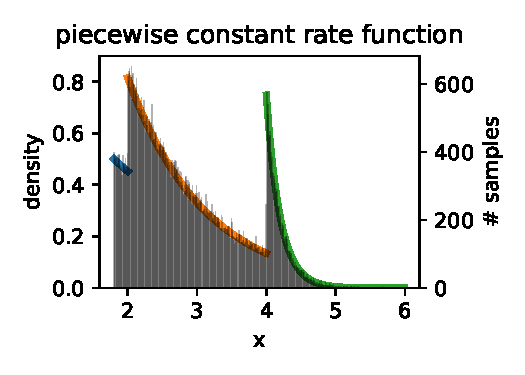
\includegraphics[width=.5\textwidth]{gfx/piecewise_c_exp.pdf}}
    \subfloat[Biased SSA simulations]
    {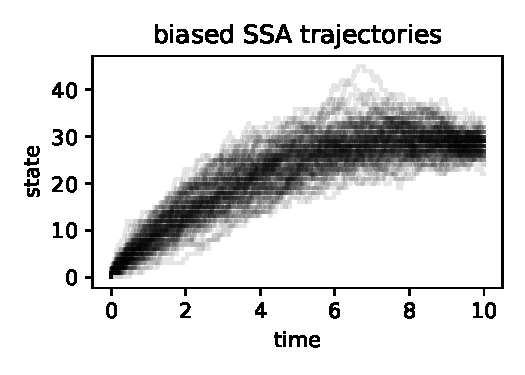
\includegraphics[width=.5\textwidth]{gfx/biased_SSA.pdf}}
    \caption[Bias interpolation \& biased \ac{SSA}]{\label{fig:bias_ssa}}
    \caption[Importance Sampling using piecewise constant jump distributions]{Importance Sampling using piecewise constant jump distributions: (a) A piecewise constant rate function is induced by the biases changing at discrete time points. (b) We can simulate the system using piecewise constant biases.}
\end{figure}

%\begin{figure}[htb]
    %\centering
    %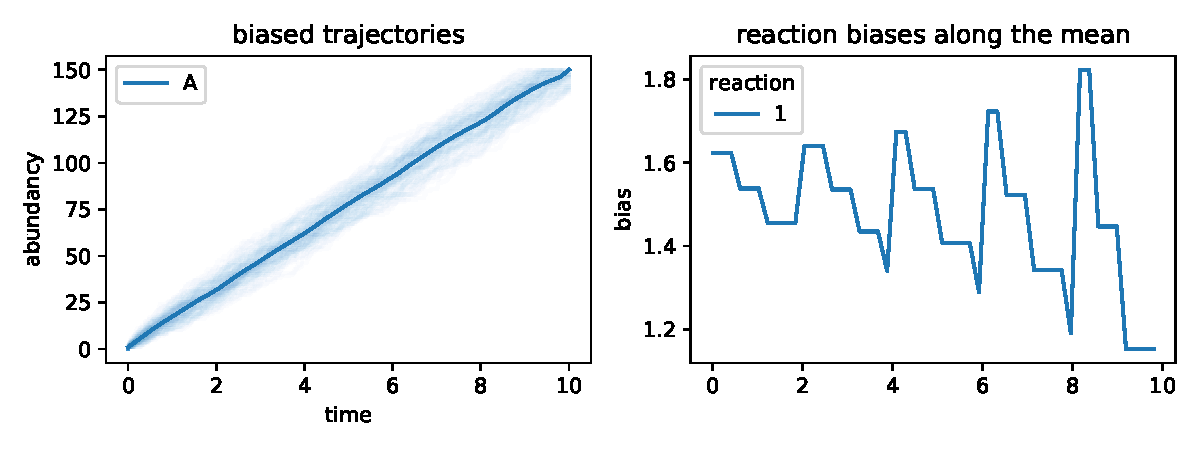
\includegraphics[width=\textwidth]{gfx/poisson_sims_and_biases.pdf}
    %\caption[Dynamic biasing for the Poisson process]{\label{fig:poisson_rare}The dynamic biasing of a Poisson process with rate 10 based on a lumping of \num{10} states.}
%\end{figure}

\begin{figure}[htb]
    \centering
    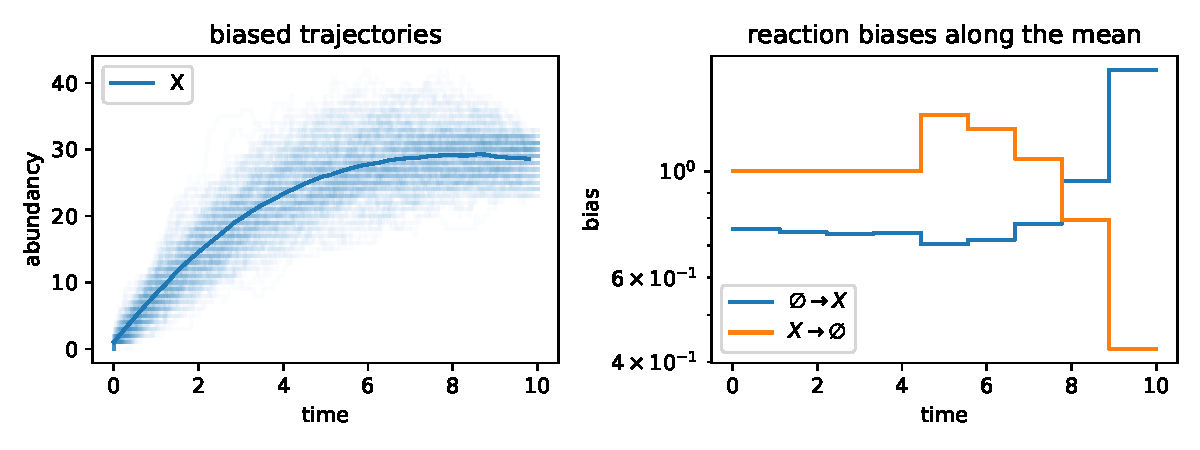
\includegraphics[width=\textwidth]{gfx/bd_is.pdf}
    \caption[Dynamic biasing for the Poisson process]{\label{fig:bd_rare}The dynamic biasing of a birth-death process lumping of \num{10} states and the target event $X(10)=30$.}
\end{figure}
\section{Case Studies}
We implemented the methods in Python and evaluated the method on three case studies.
The first two are rather simple, but have the advantage of a known analytical distribution.
Thus, we have a reference to compare the Monte Carlo results.
In the second part, we take a look at a more challenging model -- the toggle switch.
In this example, we face non-polynomial rate functions and a bi-modal behavior.
\subsection{Two Simple Examples}
For the Poisson process we look at the event of exceeding a threshold of \num{150} before a time-horizon of $T=10$.
The lumping scheme groups \num{10} states together and records the approximate backward probabilities for \num{10} time points.
In \autoref{fig:rare_estimates:poisson}, we summarize the estimates for different sample sizes.
In this study, we observe no finite sample bias and a quick convergence to the analytical result.

In case of the birth-death process, we focus on the event of being in state \num{30} at time $T=10$.
The lumping scheme groups \num{10} states together and records the approximate backward probabilities for \num{10} time points.
In \autoref{fig:rare_estimates:birth_death}, we summarize the estimates for different sample sizes.
In this study observe no finite sample bias and a quick convergence to the analytical result.
%Here we also observe a quick convergence to the analytical result.
\begin{figure}[htb]
    \centering
    \subfloat[Poisson process]
    {\label{fig:rare_estimates:poisson}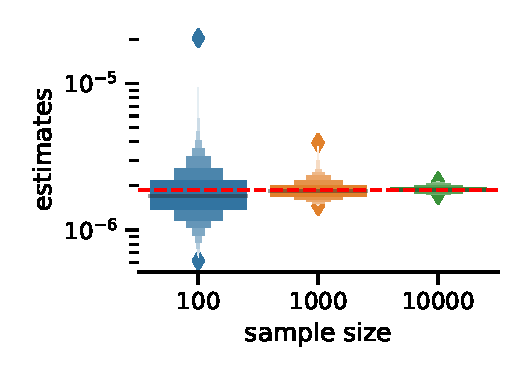
\includegraphics[width=.5\textwidth]{gfx/poisson_estimates.pdf}}
    \subfloat[Birth-death bridge]
    {\label{fig:rare_estimates:birth_death}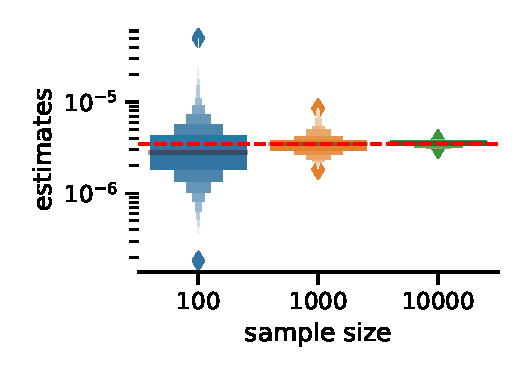
\includegraphics[width=.5\textwidth]{gfx/bridge_estimates.pdf}}
    \caption[Estimate distribution for different sample sizes]{\label{fig:rare_estimates}Estimate distribution for different sample sizes.}
\end{figure}
\subsection{Toggle Switch}
We return to the example of the toggle switch, known from \autoref{ch:bridging}.
It notably includes two non-polynomial propensity functions.
\begin{model}[Toggle Switch using Hill functions~\parencite{lipshtat2006genetic}]\label{model:hill_toggle_rare}
We have population types $A$ and $B$ with the following reactions and reaction rates.
$$ \varnothing \xrightarrow{\alpha_1(\cdot)} A\,,\quad \text{where}\quad \alpha_1(x) = \frac{\rho}{1 + k x_B},
\qquad A \xrightarrow\lambda \varnothing $$
$$ \varnothing \xrightarrow{\alpha_1(\cdot)} B\,,\quad \text{where}\quad \alpha_1(x) = \frac{\rho}{1 + k x_A},
\qquad B \xrightarrow\lambda \varnothing $$
The parameterization is $\rho=10$, $\lambda=0.1$, and $k=1.5$.
\end{model}
The sums of non-polynomial propensity functions have no simple analytical solution as the Faulhaber formulae.
Instead, we approximate the discrete sums via an integral:
\[
\begin{split}
    \bar{\alpha}_1(\bar{x})&\approx\int_{a-0.5}^{b+0.5} \frac{\rho}{1 + kx}\, dx\\
    &= \frac{\rho}{k} \left(\log{\left(k\left(b - \frac{1}{2}\right) + 1\right)} - \log{\left(k\left(a + \frac{1}{2}\right) + 1 \right)} \right)
\end{split}
\]
In this case study, we use both, a aggregation of $5\times 5$ and $10\times10$ states.
As an initial state we fix $(100, 0)$ and the target event is
\(\{X_t^{(B)} \geq 100 \mid t\leq 10 \}\).
In \autoref{fig:hill_rare}, we illustrate the sample trajectories and their mean under the biasing of the approximate backward probabilities.
On the left-hand side, the mean bias is given over time and per reaction.
The biasing strength increases towards the time-horizon.
\begin{figure}[htb]
    \centering
    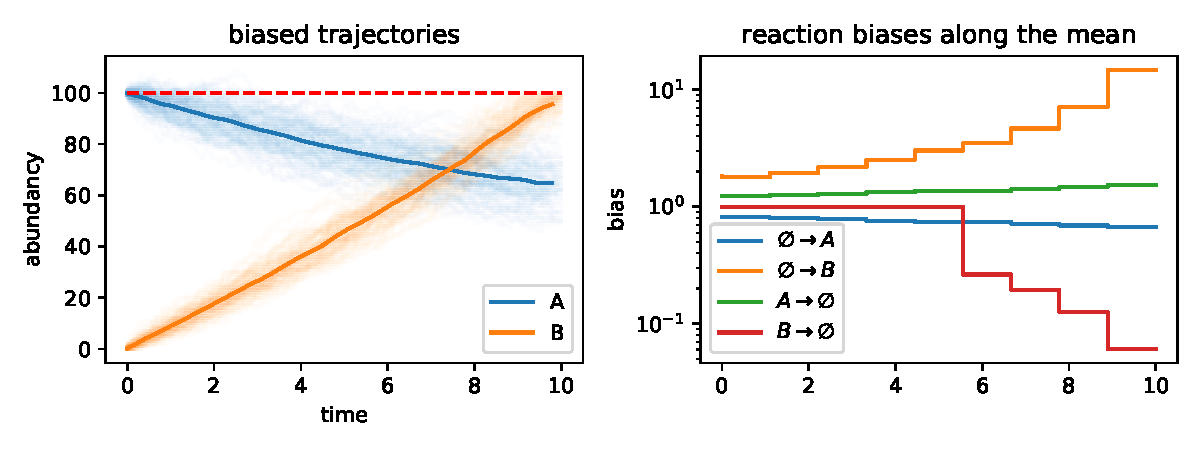
\includegraphics[width=\textwidth]{gfx/hill_toggle_is.pdf}
    \caption[Dynamic biasing for the toggle switch]{\label{fig:hill_rare}The dynamic biasing of a toggle switch based on a lumping of $10\times 10$ states.}
\end{figure}

In \autoref{fig:hill_estimates}, we provide estimates for this case study using the aggregation-based approach presented here and the popular \acsfont{dwSSA} method as a point of comparison.
\acsfont{dwSSA} \cite{daigle2011automated} essentially derives a constant bias coefficient for each reaction.
The biases are optimizes using a cross-entropy objective.
This optimization, however, needs a large number of runs in each iteration.
We used ensemble sizes of \num{1000} and \num{10000} for each iteration.
This imposes a large additional cost, since in almost all instances more than \num{10} optimization iterations were necessary, until a fraction of $0.1$ ensemble trajectories reached the rare event region.
In some instances no change of measure was found using the cross-entropy optimization.
\begin{figure}[htb]
    \centering
    \begin{minipage}{0.77\textwidth}
        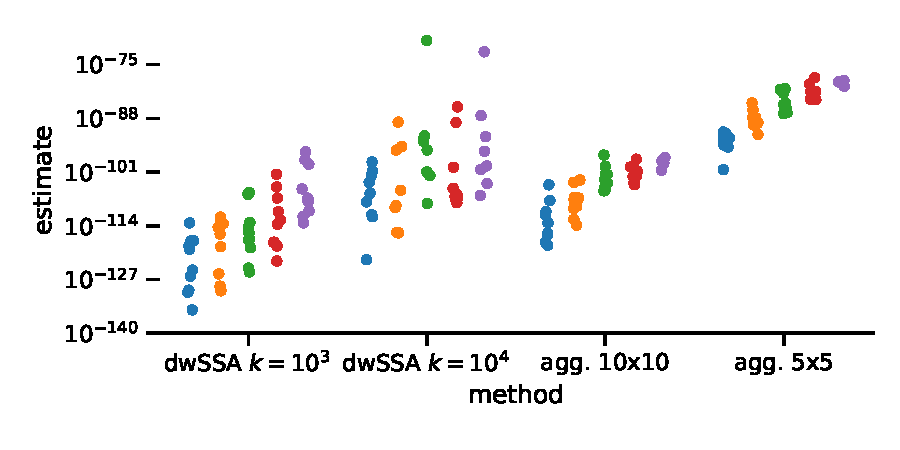
\includegraphics[scale=.55]{gfx/hill_estimates.pdf}
    \end{minipage}
    \hspace{1ex}
    \begin{minipage}{0.07\textwidth}
        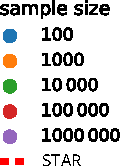
\includegraphics[scale=.55]{gfx/hill_estimates_legend.pdf}
    \end{minipage}
    \caption[Rare event estimates (toggle switch)]{\label{fig:hill_estimates}Rare event estimates (toggle switch with Hill functions) using different methods and sample sizes. For each scenario \num{10} estimations were performed. To the left are the \acsfont{dwSSA} results for comparison. We provide results for estimates using \num{1000} and \num{10000} estimates in each iteration of the prior parameter optimization rounds. On the right, the results for the aggregation method presented in this chapter are given for grids with $5\times 5$ and $10\times 10$ macro states.}
\end{figure}

%\begin{itemize}
    %\item more likely paths are sampled less often
    %\item sample weight distribution not normal
    %\item a high-weight tail
    %\item still unbiased, but too large ``outliers'' need to correct for many estimates that are too low. therefore many samples are necessary
    %\item less variance in agg. because paths are steared more (not better estimates though...)
%\end{itemize}
With both methods, we observe that with smaller sample sizes, the estimate tends to be smaller as well, regardless of the method.
This is due to the (non-zero) weights not being normally distributed.
There tend to be more samples with lower weight, which are compensated by few samples with a marger larger weight.
In other words, there seems to be a long tail towards to higher weights in most cases.
The theoretical estimate is still unbiased.
But the estimates which are much larger (``correcting'' the low estimates) are very infrequent.
This issue is present regardless of the chosen method.
The most clear difference is that the estimates using aggregation are spread less.
This effect is likely due to the aggregation-based biasing steering the process with more detail.
Therefore trajectories tend to be more similar --- an effect that is also appearant in the samples of \autoref{fig:hill_paths_comp}.

As a reference and baseline we consider the dynamic truncation result obtained by the \acsfont{STAR} tool \parencite{lapin2011shave}.\marginpar{\url{mosi.uni-saarland.de/tools/shave/}}
We ran the analysis using a relative tolerance of \num{1e-15} and an absolute tolerance of \num{1e-90}.
This yielded \(\Pr(X_{10}^{(B)} \geq 100) \approx \num{4.64e-60}\).
Note, that this is a lower bound to the probability since we only consider the probability at $t=10$, whereas the stopping time above considers all $t\leq 10$.
Considering this baseline, it is clear, that both methods have only slowly approach the probability's true magnitude with increasing sample size.

%\begin{itemize}
    %%\item different areas sampled
    %\item right: low weights if B increases early or A does not decrease in the end (tendency)
    %\item right: large variance in sample weights (orders of magnitude)
    %\item left: weights are closer together
    %\item conclusion: sampling true transition paths may require more than constant biasing
%\end{itemize}
In \autoref{fig:hill_paths_comp}, we compare sample paths using the technique presented here with a constant biasing scheme. 
The constant biases are obtained using a cross-entropy optimization using $10^4$ \ac{SSA} simulations in each iteration until $0.1$ of the trajectories reach the rare event region.
It is immediately clear, that the sampled trajectories differ in the paths that are sampled.
%The theoretical optimal sampling would generate trajectories proportional to the original system dynamics conditioned on reaching reaching the rare event.
We further observe a far larger range of likelihood ratios in the constant biasing case.
\begin{figure}[htb]
    \centering
    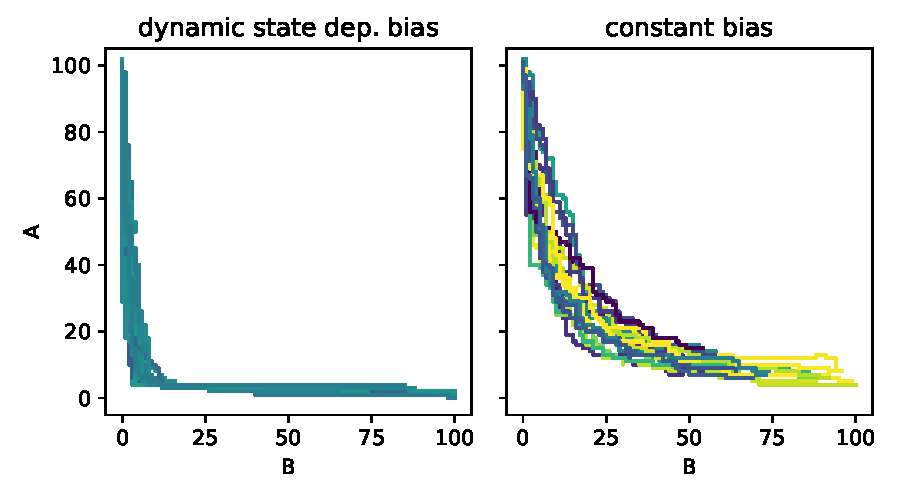
\includegraphics[scale=.6]{gfx/hill_paths_comp.pdf}
    \caption[Comparison of biased sample paths]{\label{fig:hill_paths_comp}Biased sample paths of the toggle switch using (left) the aggregation based sampling and (right) a constant biasing, determined by cross-entropy optimization \parencite{daigle2011automated}. The constant bias vector is $\approx (0.873, 26.248, 2.751, 0.00159)^{\top}$. The path color represents the relative $\log$ weghts of each trajectory (darker -- higher weight).}
\end{figure}

This case study showcases the major difficulty in finding an efficient change of measure that one can encounter.
Ideally, sampled trajectories should follow the original process, conditioned on the rare event.
As in this example, constant biases might not be enough to reliably alter the dynamics in this way.
However, the approximate biasing scheme presented in this chapter, while being based on an approximation of the ideal biasing, seems to over-constrain the process and thus not explore the trajectory space sufficiently.
Consequently, both methods tend to under-estimate in a majority of cases.

\section{Conclusion}
In this chapter, we presented a novel change of measure using approximate backward probabilities.
This approach avoids the necessity of a significant number of pilot runs.
In the last example, the number of these pilot runs often exceeded the number of runs used for the estimate.
Therefore, the approach presented is a feasible alternative for cases in which the state-space size allows for an approximate solution.

We further showcased a challenge that is often emphasized too little.
This is the issue of changes of measures, that steer the process to the target region along trajectories that are significantly less likely in the original system than the conditioned paths would be.
This leads to a case where the estimate distribution is very different from a normal distribution.
Consequently, the estimates are too low in most cases, and a lot too large in very few cases.

This issue might be tackled by, using state space refinement, similar to the previous chapter.\turnto{ch:bridging}
Also, combining  backward probability approximations of differing granularity might be a viable strategy.
%\paragraph{Issues}
%\begin{itemize}
    %\item emphasize large cost of pilot runs
    %\item due to the approximative nature, the speed is often too high or too low
    %\item simultions reach the target to early: many samples with very low weight, few with high weight
    %\item the estimates are still unbiased but not approximately normally distributed, even for larger biases (make an example, that this is also the case for constant biasing)
    %\item bias strength can be adjusted such that only a portion reaches
    %\item this improves the somewhat, but may alter the biases too much and the weight distribution (sampled) is still bad
%\end{itemize}
%\paragraph{Future Work}
%\begin{itemize}
    %\item \emph{Multiple importance sampling} for different accelerations to avoid problems of under- and overacceleration
%\end{itemize}
